% ME 3001 - Tristan Hill - Summer 2016 - Spring 2024
% The Eigenvalue Problem and Vectors
% Weekly Problem 4


% Document settings
\documentclass[11pt]{article}
\usepackage[margin=1in]{geometry}
\usepackage[pdftex]{graphicx}
\usepackage{multirow}
\usepackage{setspace}
\usepackage{hyperref}
\usepackage{color,soul}
\usepackage{fancyvrb}
\usepackage{framed}
\usepackage{wasysym}

\pagestyle{plain}
\setlength\parindent{0pt}
\hypersetup{
    bookmarks=true,         % show bookmarks bar?
    unicode=false,          % non-Latin characters in Acrobat’s bookmarks
    pdftoolbar=true,        % show Acrobat’s toolbar?
    pdfmenubar=true,        % show Acrobat’s menu?
    pdffitwindow=false,     % window fit to page when opened
    pdfstartview={FitH},    % fits the width of the page to the window
    pdftitle={My title},    % title
    pdfauthor={Author},     % author
    pdfsubject={Subject},   % subject of the document
    pdfcreator={Creator},   % creator of the document
    pdfproducer={Producer}, % producer of the document
    pdfkeywords={keyword1} {key2} {key3}, % list of keywords
    pdfnewwindow=true,      % links in new window
    colorlinks=true,       % false: boxed links; true: colored links
    linkcolor=red,          % color of internal links (change box color with linkbordercolor)
    citecolor=green,        % color of links to bibliography
    filecolor=magenta,      % color of file links
    urlcolor=blue           % color of external links
}

% assignment number 
\newcommand{\NUM}{4} 

\definecolor{mygray}{rgb}{.6, .6, .6}

\setulcolor{red} 
\setstcolor{green} 
\sethlcolor{mygray} 

\begin{document}

	\textbf{\LARGE ME 3001, Spring 2024} \\\\
	\textbf{\LARGE Weekly Problem \NUM: Eigenvalues and Eigenvectors} \\\\
		
		\textbf{\large Complete the following regarding the Eigenvalue Problem for 2D vectors.}\\\\


              \begin{enumerate}

\item Given: $ [A]=\left[ \begin{array}{cc} 3 & 2  \\ 3 & -2   \end{array} \right], $ \hspace{10mm} $ \{v\}=\left\{ \begin{array}{c} 4 \\ 2   \end{array} \right\} $, and $ \{u\}=\left\{ \begin{array}{c} -3 \\ 1   \end{array} \right\} $ \\\\\\
Find:  $\{v'\}=[A]\{v\}$ and  $\{u'\}=[A]\{u\}$ \vspace{20mm}\\


\item Sketch all 4 vectors ($v,v',u,u'$) on the graph paper given to scale as best as possible.  \vspace{00mm}\\

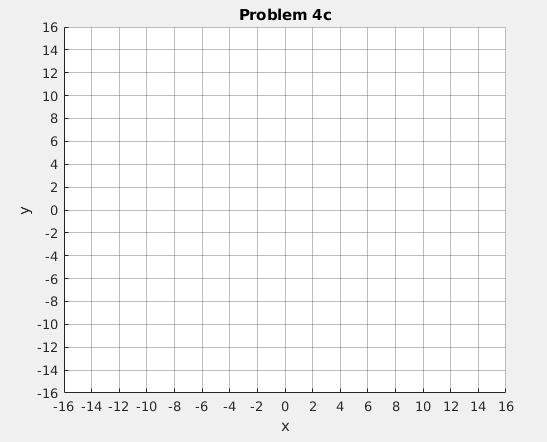
\includegraphics[scale=.6]{exam1_prob4c.png}
%\includegraphics[scale=.35]{quiz3_fig1.png}
\item Is either $\{v\}$ or $\{u\}$ an Eigenvector of $[A]$? If so what is the Eigenvalue?\\\\

\item Find the second Eigenvalue of $[A]$ as well as 1 Eigenvector associated with it.

\end{enumerate}		



\end{document}



